%%%%%%%%%%%%%%%%%%%%%%%%%%%%%%%%%%%%%%%%%
% Dreuw & Deselaer's Poster
% LaTeX Template
% Version 1.0 (11/04/13)
%
% Created by:
% Philippe Dreuw and Thomas Deselaers
% http://www-i6.informatik.rwth-aachen.de/~dreuw/latexbeamerposter.php
%
% This template has been downloaded from:
% http://www.LaTeXTemplates.com
%
% License:
% CC BY-NC-SA 3.0 (http://creativecommons.org/licenses/by-nc-sa/3.0/)
%
%%%%%%%%%%%%%%%%%%%%%%%%%%%%%%%%%%%%%%%%%

%----------------------------------------------------------------------------------------
%	PACKAGES AND OTHER DOCUMENT CONFIGURATIONS
%----------------------------------------------------------------------------------------

\documentclass[final,hyperref={pdfpagelabels=false}]{beamer}

\usepackage[orientation=portrait,size=a0,scale=0.94]{beamerposter} % Use the beamerposter package for laying out the poster with a portrait orientation and an a0 paper size

\usetheme{I6pd2} % Use the I6pd2 theme supplied with this template

\usepackage[english]{babel} % English language/hyphenation

\usepackage{amsmath,amsthm,amssymb,latexsym} % For including math equations, theorems, symbols, etc

%\usepackage{times}\usefonttheme{professionalfonts}  % Uncomment to use Times as the main font
%\usefonttheme[onlymath]{serif} % Uncomment to use a Serif font within math environments

\usepackage{graphicx}
\usepackage{framed}
\usepackage{mathtools}
\DeclarePairedDelimiter{\floor}{\lfloor}{\rfloor}

\boldmath % Use bold for everything within the math environment

\usepackage{booktabs} % Top and bottom rules for tables

\graphicspath{{figures/}} % Location of the graphics files

\usecaptiontemplate{\small\structure{\insertcaptionname~\insertcaptionnumber: }\insertcaption} % A fix for figure numbering

%----------------------------------------------------------------------------------------
%	TITLE SECTION 
%----------------------------------------------------------------------------------------

\title{\huge Robust Virtual Scan for Obstacle Detection in Urban Environments} % Poster title

\author{Mengwen He$^{1,3}$, Eijiro Takeuchi$^{1}$, Yoshiki Ninomiy$^{2,3}$, and Shinpei Kato$^{1,3}$} % Author(s)

\institute{$^1$Graduate School of Information Science, Nagoya University\\
	$^2$Institute of Innovation for Future Society (MIRAI), Nagoya University\\
	$^3$JST/COI, Nagoya} % Institution(s)

%----------------------------------------------------------------------------------------
%	FOOTER TEXT
%----------------------------------------------------------------------------------------

\newcommand{\leftfoot}{http://www.coi.nagoya-u.ac.jp/} % Left footer text

\newcommand{\rightfoot}{alexanderhmw@gmail.com} % Right footer text

%----------------------------------------------------------------------------------------

\begin{document}

\addtobeamertemplate{block end}{}{\vspace*{2ex}} % White space under blocks

\begin{frame}[t] % The whole poster is enclosed in one beamer frame

\begin{columns}[t] % The whole poster consists of two major columns, each of which can be subdivided further with another \begin{columns} block - the [t] argument aligns each column's content to the top

\begin{column}{.02\textwidth}\end{column} % Empty spacer column

\begin{column}{0.47\textwidth} % The first column

%----------------------------------------------------------------------------------------
%	OBJECTIVES
%----------------------------------------------------------------------------------------

\begin{block}{Objectives}

\begin{itemize}
\item Develop a robust and real-time algorithm to transfer the point-cloud captured by a 3D LiDAR (e.g. Velodyne) to a 2D virtual scan (VScan) to represent the obstacles around the ego-vehicle. (Fig. \ref{fig:vscan})
\item Handle the inefficiency of general VScan methods on conditions of sloped roads (e.g. steep ramp), small objects (e.g. road curb), and overhung obstacles (e.g. barrier gate). (Fig. \ref{fig:challenge})
\end{itemize}

\begin{figure}
	\centering
	\includegraphics[width=\textwidth]{vscan}
	\caption{Transfer the 3D point-cloud to a 2D virtual scan. The word "virtual" means that the scan is not from a real 2D LiDAR but from the input 3D point-cloud; therefore, we can find an undetected area in this figure, which is a dead zone for our vehicle-borne Velodyne.}
	\label{fig:vscan}
\end{figure}

\begin{figure}
	\centering
	\includegraphics[width=\textwidth]{challenge}
	\caption{Challenging scenarios for general VScan methods. The road surface of steep ramp would be falsely detected as an obstacle; The road curb and barrier gate would be ignored as free space.}
	\label{fig:challenge}
\end{figure}

\end{block}

%----------------------------------------------------------------------------------------
%	INTRODUCTION
%----------------------------------------------------------------------------------------
            
\begin{block}{Introduction}

\begin{itemize}
\item Many intelligent vehicles rely on LiDARs for obstacle detection as well as localization and mapping.
\item The 3D LiDAR, e.g. Velodyne, can fully scan the real world at 10 Hz producing nearly 100,000 points per frame; however, directly processing a frame of point-cloud is always time-consuming.
\item The 2D LiDAR, e.g. SICK or Hokuyo, can horizontally scan the surrounding and briefly represent the obstacles as an array of range values; however, it may falsely detect sloped road surfaces as obstacles, and it cannot properly detect low or overhung obstacles.
\item The VScan is also an array of range values from a 2D compact transformation of point-cloud. Meanwhile, we developed a robust and real-time VScan algorithm to handle the sloped road, low objects and overhung obstacles. Therefore, the VScan is suitable for rapid further processing in a complex urban environment.
\end{itemize}

\end{block}

\begin{block}{Contributions}

\begin{itemize}
	\item A new data structure called \textit{Basic VScan Matrix} (BVSM) represents point-cloud around the ego-vehicle.
	\item A \textit{Simultaneous Road Filtering and Obstacle Detection} (SRFOD) algorithm works on top of BVSM for robust VScan generation (mainly focuses on slope roads, low objects, and overhung obstacles).
	\item A \textit{Sorted Array based Acceleration Method} (SAAM) enables real-time VScan generation.
\end{itemize}

\end{block}

%----------------------------------------------------------------------------------------
%	METHODS
%----------------------------------------------------------------------------------------

\begin{block}{Method Description}

\begin{columns}
	\begin{column}{0.46\textwidth}
		\begin{figure}
			\centering
			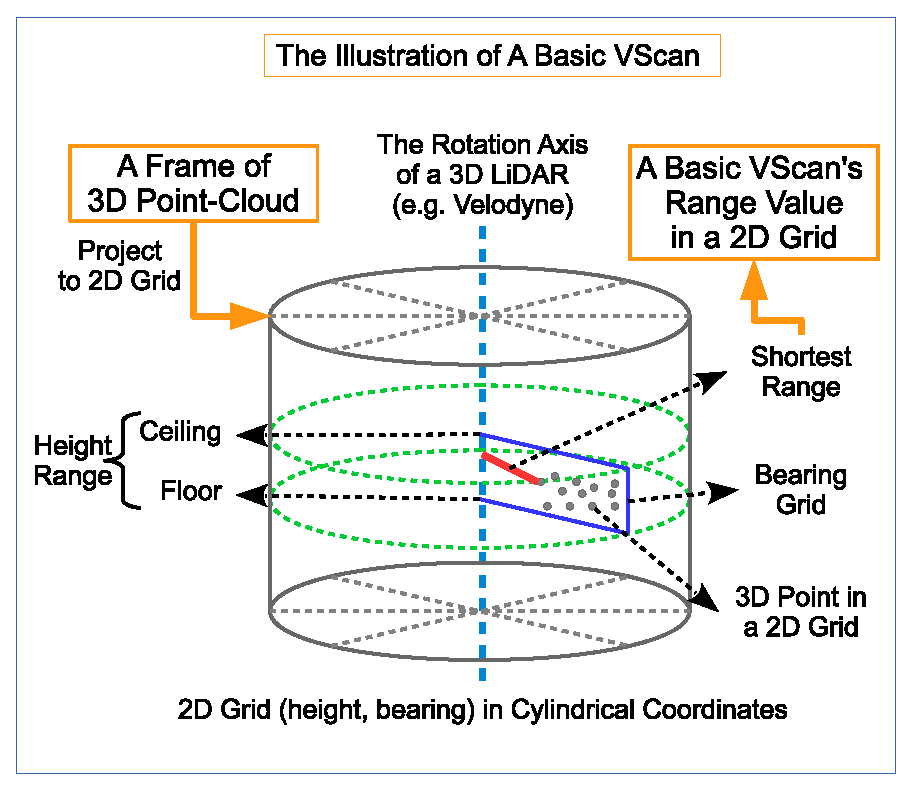
\includegraphics[width=\textwidth]{grid}
			\caption{The basic VScan is normally extracted from a chosen set of points within a height range (Floor $\rightarrow$ Ceiling), and its range value in each bearing grid is calculated as the shortest range between the axis and the points.}
		\end{figure}
	\end{column}
	
	\begin{column}{0.46\textwidth}
		\begin{figure}
			\centering
			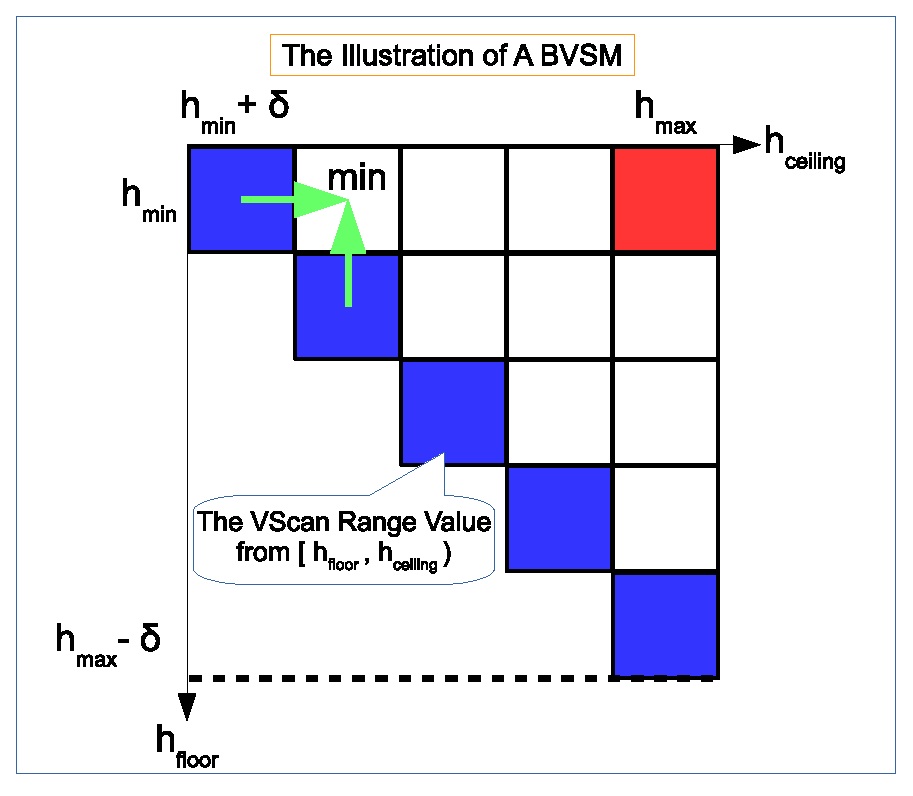
\includegraphics[width=\textwidth]{BVSM}
			\caption{A BVSM collects all possible Basic VScans' range values in the same bearing grid. The blue diagonal cells correspond to the minimum height range $\delta$, and the off-diagonal cells can be calculated via $min$ operation (the green arrows).}
		\end{figure}
	\end{column}
\end{columns}

\begin{center}
	\begin{column}{0.97\textwidth}
		\begin{figure}
			\centering
			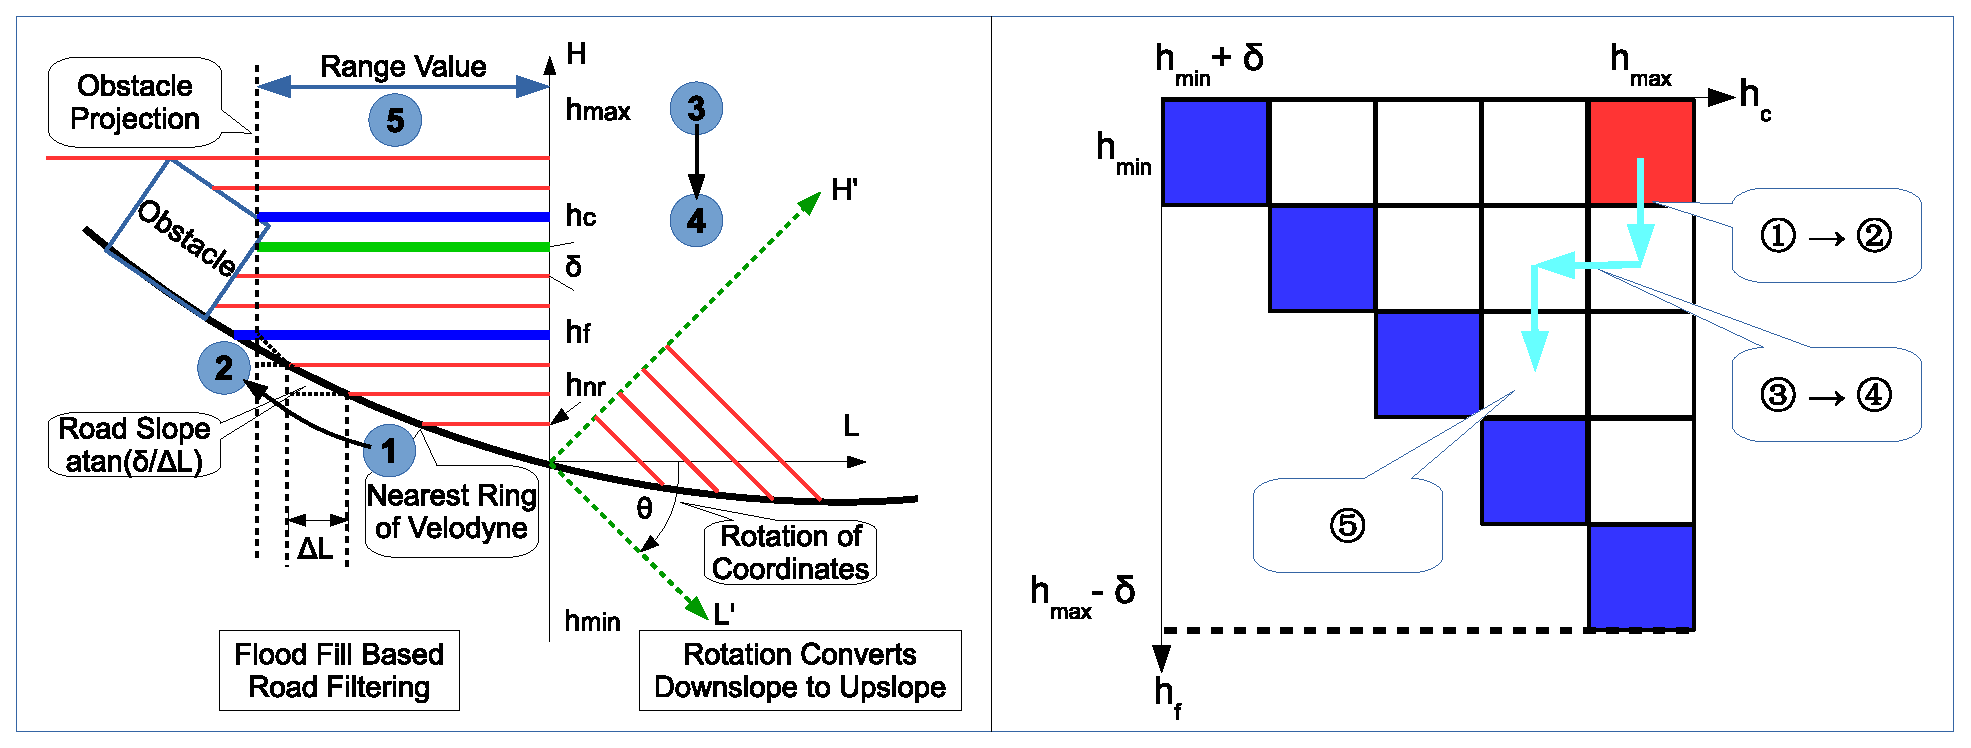
\includegraphics[width=\textwidth]{SRFOD}
			\caption{The SRFOD is to find a proper height range ($h_f \rightarrow h_c$) starting from the max height range ($h_{min} \rightarrow h_{max}$) for basic VScan calculation as well as obstacle detection in each bearing grid. [Left] $\textcircled{1} \rightarrow \textcircled{2}$ (road filtering stage): use the flood fill method with slope threshold to filter road surface. $\textcircled{3} \rightarrow \textcircled{4}$ (obstacle detection stage): lower ceiling to filter fake obstacles highly elevated above the ground. $\textcircled{5}$: after several alterations between these two stages, the proper height range is determined, and the range value is from the corresponding basic VScan. [Right] The SRFOD process can be represented as the movement (the cyan path) from the red corner cell toward the blue diagonal cells on the BVSM. The movement decision is presented in the following "Algorithm Description" section. Additionally, the SRFOD cannot work on downslope roads; therefore, we use a temporary rotation, which keeps geometry consistency, to convert a downslope road to an upslope road for obstacle detection, and then revert this rotation to determine the final range value.}
		\end{figure}
	\end{column}
\end{center}



\end{block}

%----------------------------------------------------------------------------------------

\end{column} % End of the first column

\begin{column}{.02\textwidth}\end{column} % Empty spacer column
 
\begin{column}{.48\textwidth} % The second column


%----------------------------------------------------------------------------------------
%	Algorithm SECTION
%----------------------------------------------------------------------------------------

\begin{block}{Algorithm Description}
\begin{columns}
	\begin{column}{0.49\textwidth}
		\begin{framed}
			\begin{center}
				\textbf{The BVSM Based SRFOD}
			\end{center}
			\begin{itemize}
				\item Define $L_i(h_f,h_c)$ as the range value in $i$th bearing of a basic VScan from the height interval $[h_f,h_c)$
				
				\item Index $L_i(h_f,h_c)$ as $L_i'(g_f,g_c)$:
				
				{\small\centering$\{L_i'(g_f,g_c) | g_f \in \mathbb{N}, g_c \in \mathbb{N}, g_{min} \leq g_f<g_c \leq g_{max}\}$}\\
				{\small$where~g=\floor{(h-h_{min})/\delta}$}
				
				\item Parameters:
				\begin{itemize}
					\item $\phi$: the maximum road slope.
					\item $\Delta H$: the passable height for ego-vehicle.
				\end{itemize}				
			\end{itemize}
			
			\textbf{Algorithm}:
			\begin{enumerate}
				\item Construct the BVSM of $i$th bearing grid.
				
				\item Start from $g_f=g_{min}$ and $g_c=g_{max}$.
				
				\item The rule for road or obstacle detection:
				\begin{equation}
				\label{eq:criteria}
				\small
				\Delta L \cdot tan(\phi)\left\{
				\begin{array}{cl}
				\geq\delta & \Rightarrow Road \\
				<\delta & \left\{
				\begin{array}{cl}
				\Delta h > \Delta H & \Rightarrow Unknown \\
				\Delta h \leq \Delta H & \Rightarrow Obstacle
				\end{array}
				\right.
				\end{array}
				\right. 
				\end{equation}
				{where\\ \small$\Delta L = L'_i(g_f+1,g_c)-L'_i(g_f,g_c)\geq0$, and \\$\Delta h=h_c-h_f$}
				
				\item The decision of next movement on the BVSM:
				\begin{itemize}
					\small
					\item Road: move to cell $(g_f+1,g_c)$ (down, \textcircled{1} $\rightarrow$ \textcircled{2}).
					\item Unknown: move to cell $(g_f,g_c-1)$ (left, \textcircled{3} $\rightarrow$ \textcircled{4}). 
					\item Obstacle: stop, and $L'_i(g_f,g_c)$ is the final result (\textcircled{5}).
				\end{itemize}
				
				\item Goto step 3 until $g_f+1=g_c$.
			\end{enumerate}
			
			\textbf{Complexity Analysis}:
			\begin{itemize}
				\item Parameters:
				\begin{itemize}
					\item $P$: the number of 3D points.
					\item $N$: bearing grid number (range array length).
					\item $M$: height grid number ($(h_{max}-h_{min})/\delta$).
				\end{itemize}
				\item Computational Complexity: $O(P+NM^2)$
				\begin{itemize}
					\item BVSMs' diagonal cells: $O(P)$
					\item BVSMs' off-diagonal cells: $O(NM^2)$
					\item SRFOD on BVSMs: $O(NM)$
				\end{itemize}
			\end{itemize}
			\textbf{Problem}: If the high resolution of height grid (small $\delta$) is required for low objects detection, the large $M$ makes this algorithm time-consuming.
			\vspace{0.2em}
		\end{framed}
	\end{column}
		
		\begin{column}{0.49\textwidth}
			\begin{framed}
				\begin{center}
					\textbf{The SAAM}
				\end{center}
				\begin{itemize}
					\item The construction of BVSMs costs too much time and memory space; however, the BVSMs' off-diagonal cells can be directly derived from their sorted diagonal cells (see the property C in this paper's appendix).
					\item The SAAM will only use the BVSMs' sorted diagonal cells to realize SRFOD; therefore, it can significantly accelerate the SRFOD when the height grid number ($M$) is large.
				\end{itemize}
				
				\textbf{Algorithm}:
				\begin{enumerate}
					\item Calculate the diagonal cells ($\{L_i'(g_f,g_f+1)\}$) of the BVSM of $i$th bearing grid.
					\item Sort diagonal cells in ascending order and for the cells have same $L_i'$, sort them with their floor height index $g_f$ in descending order. After sorting, we get two associated arrays: $L_i'[j]$ and $g_f[j]$.
					\item Start from $j_0=0$ and $j_1=1$.
					\item The rule for road or obstacle detection:
					\small
					\begin{equation*}
					\Delta g
					\left\{
					\begin{array}{cl}
					<0 & \Rightarrow Unknown \\
					=1 & \Rightarrow (\ref{eq:criteria}) \\
					>1 & \left\{
					\begin{array}{cl}
					\Delta h > \Delta H & \Rightarrow Unknown \\
					\Delta h \leq \Delta H & \Rightarrow (\ref{eq:addcriteria})
					\end{array}
					\right.
					\end{array}
					\right.
					\end{equation*}
					\begin{equation}
					\label{eq:addcriteria}
					\Delta L \cdot tan(\phi)\left\{
					\begin{array}{cl}
					<\delta & Obstacle \\
					\geq\delta & Obstacle*  
					\end{array}
					\right. 
					\end{equation}
					$\Delta L = L'_i[j_1] - L'_i[j_0]$, $\Delta h = h_f[j_1]-h_f[j_0]$, and $\Delta g = g_f[j_1]-g_f[j_0]$ 
					
					\item The decision of next movement on the sorted array:
					\begin{itemize}
						\small
						\item Road: $j_0 \leftarrow j_1$ and $j_1 \leftarrow j_1+1$.
						\item Unknown: $j_1 \leftarrow j_1+1$.
						\item Obstacle: stop, and $L'_i[j_0]$ is the final result.
						\item Obstacle*: stop, and $L'_i[j_1]$ is the final result.
					\end{itemize}
					
					\item Goto step 4 until $j_1$ exceeds the sorted array range.
				\end{enumerate}
				
				\textbf{Computational Complexity}: $O(P+NM\log(M))$
				\begin{itemize}
					\item BVSMs' diagonal cells: $O(P)$
					\item Sort diagonal cells of each BVSM: $O(NM\log(M))$
					\item SRFOD on the sorted arrays: $O(NM)$
				\end{itemize}
			\end{framed}
		\end{column}
\end{columns}

\begin{itemize}
	\item Speed test with $P\approx100,000$, $N=2000$, and $\delta=0.05m \Rightarrow M=100$ (Intel Xeon ES-1660 3.70GHz):
	\begin{itemize}
		\item The BVSM based SRFOD costs $113ms>100ms$, and Velodyne's working frequency is $10Hz$.
		\item The SAAM costs $13ms$, and it is suitable for real-time applications. 
	\end{itemize}
\end{itemize}


%\begin{columns}
%	\begin{column}{0.4\textwidth}
%		\begin{itemize}
%			\item 
%		\end{itemize}
%	\end{column}
%	\begin{column}{0.5\textwidth}
%		\begin{figure}
%			\centering
%			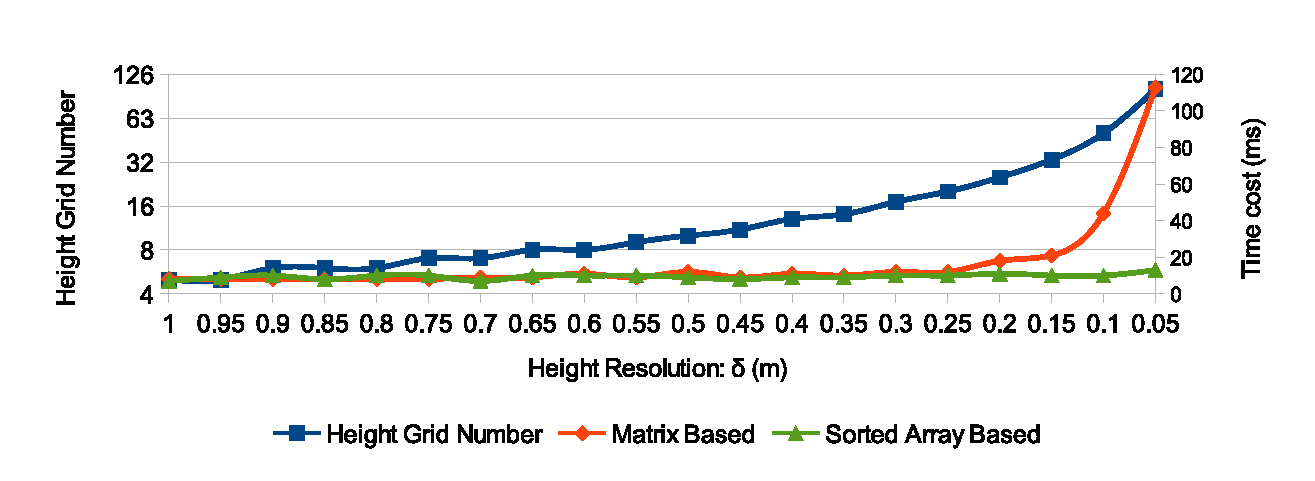
\includegraphics[width=\textwidth]{speed}
%		\end{figure}
%	\end{column}
%\end{columns}
\end{block}

\begin{block}{Further Development: 3D VScan as ``Stixels"}
	\begin{itemize}
		\item Our SRFOD method can detect the obstacle's vertical height as ``Stixels" containing min. and max. altitudes.
	\end{itemize}	
	\begin{center}
		\begin{column}{0.8\textwidth}
			\begin{figure}
				\centering
				\includegraphics[width=\textwidth]{stixel}
				\caption{The visualization of ``Stixels" (the green vertical bars) on images (first row) and in point-clouds (second row). Especially, the right column shows the detection of overhung barrier gate.}
			\end{figure}	
		\end{column}
	\end{center}
		
\end{block}

%----------------------------------------------------------------------------------------
%	Experiment RESULTS
%----------------------------------------------------------------------------------------

\begin{block}{Experiment Results$^1$}

\begin{columns}
	\begin{column}{0.573\textwidth}
		\begin{figure}
			\centering
			\includegraphics[width=\textwidth]{exp}
			\caption{[Top-Left] Our experiment vehicle Matsu equipped with a Velodyne and cameras. [Bottom-Left] The detection of low road curbs with high resolution (small $\delta$). Because the curb's height is less than $0.2m$, the road curb cannot be detected with $\delta=0.2m$. [Right] The VScan result on a steep slope road (20m long and 3m high). Our algorithm successfully filtered the slope road surface, and additionally detected a Vehicle 50m behind the ego-vehicle on a flat road.}
		\end{figure}
	\end{column}
	\begin{column}{0.36\textwidth}
		\begin{figure}
			\centering
			\includegraphics[width=\textwidth]{compare}
			\caption{We compared our method (left) with other two VScan methods$^2$: a basic implementation of F. Moosmann's depth map based method$^3$ (middle), and T. Foote's method$^4$ from ROS (right). The ego-vehicle is static, and the result accumulates 100 frames of VScan (blue$\rightarrow$red) to test its stableness.}
		\end{figure}
	\end{column}
\end{columns}

{\footnotesize\noindent-----------------------------------}\\
\begin{enumerate}
	\footnotesize
	\item More video results can be found on Youtube \url{https://youtu.be/d6l31owNs2U}.
	\item The video can be found on Youtube \url{https://youtu.be/0h0n9W6RIAQ}.
	\item F. Moosmann, O. Pink, and C. Stiller, “Segmentation of 3D lidar data in non-flat urban environments using a local convexity criterion,” in \textit{Intelligent Vehicles Symposium}, 2009 IEEE. IEEE, 2009, pp. 215–220.
	\item T. Foote, “pointcloud to laserscan ROS node.” [Online]. Available: \url{http://wiki.ros.org/pointcloud to laserscan}.
\end{enumerate}
\end{block}

%----------------------------------------------------------------------------------------
%	ACKNOWLEDGEMENTS
%----------------------------------------------------------------------------------------

\begin{block}{Acknowledgments}

\begin{itemize}
\item This research is supported by the Center of Innovation Program (Nagoya-COI: Mobility Society Leading to an Active and Joyful Life for Elderly) from Japan Science and Technology Agency.
\end{itemize}

\end{block}

%----------------------------------------------------------------------------------------

\end{column} % End of the second column

\begin{column}{.015\textwidth}\end{column} % Empty spacer column

\end{columns} % End of all the columns in the poster

\end{frame} % End of the enclosing frame

\end{document}